%\subsection{Model Validation}
\subsection{Numerical Examples}\label{sec:hierarchical:analyticbw:results}

We evaluate the performance of tiered caching systems with bandwidth constraints in parameter studies.
We validate the model via simulations, which allows us to verify the accuracy of the analytical model and the validity of our conclusions based on the model for a wide range of system parameters.
Before presenting numerical examples, we briefly describe the event-based simulation.
%We compare the results derived from our analytical models with results derived by event-based simulation.
The simulation framework used is implemented in Matlab and described in detail in \cite{info3-inproceedings-2015-530}. The results presented show the mean values of 8 runs with 95\% confidence intervals, each run simulating $10^5$ requests in the stationary phase.

If not stated otherwise, in the remainder of this study, the catalogue size is $N=1e6$.
The number of tier-1 caches is $n_1=1e4$, each having a capacity of $C_1=8$.
There is one tier-2 cache with default capacity $C_2=1e4$.
The tier-1 cache upload bandwidth is limited to $0.8Mbps$, whereas the tier-2 cache has unlimited upload bandwidth.

%\begin{itemize}
%	\item Methodology
%	\item Performance metrics \\
%    - cache capacity of ISP cache necessary to replace home routers
%	\item Results
%  \item upper bound wrt uploadrate optimal case, always hit in tier 2
%  \item Optimal strat dependent on AS size and HG capacity
%  \item Optimization -> LCP with P ~ overlay distribution
%   \item request rate proportional AS size -> HWC
%\end{itemize}

\begin{figure*}[bt]
\begin{minipage}[t]{0.49\textwidth}
  \centering
  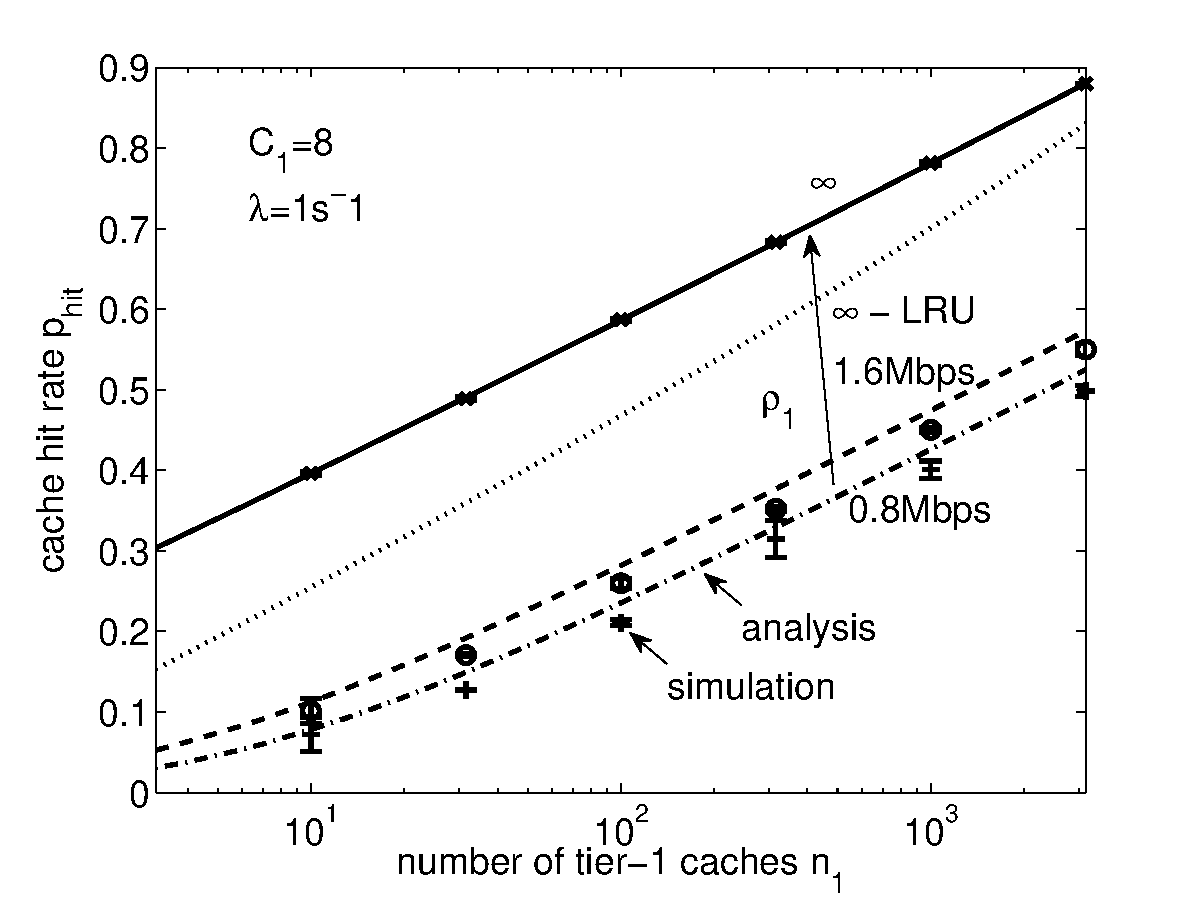
\includegraphics[width=\textwidth]{hierarchical/analyticbw/figures/hwc_CISP0}
  \caption{Comparison of cache hit rate for optimal placement with LRU policy.}
  \label{fig:hwc_CISP0}
\end{minipage}
\hspace{0.01\textwidth}
\begin{minipage}[t]{0.49\textwidth}
  \centering
  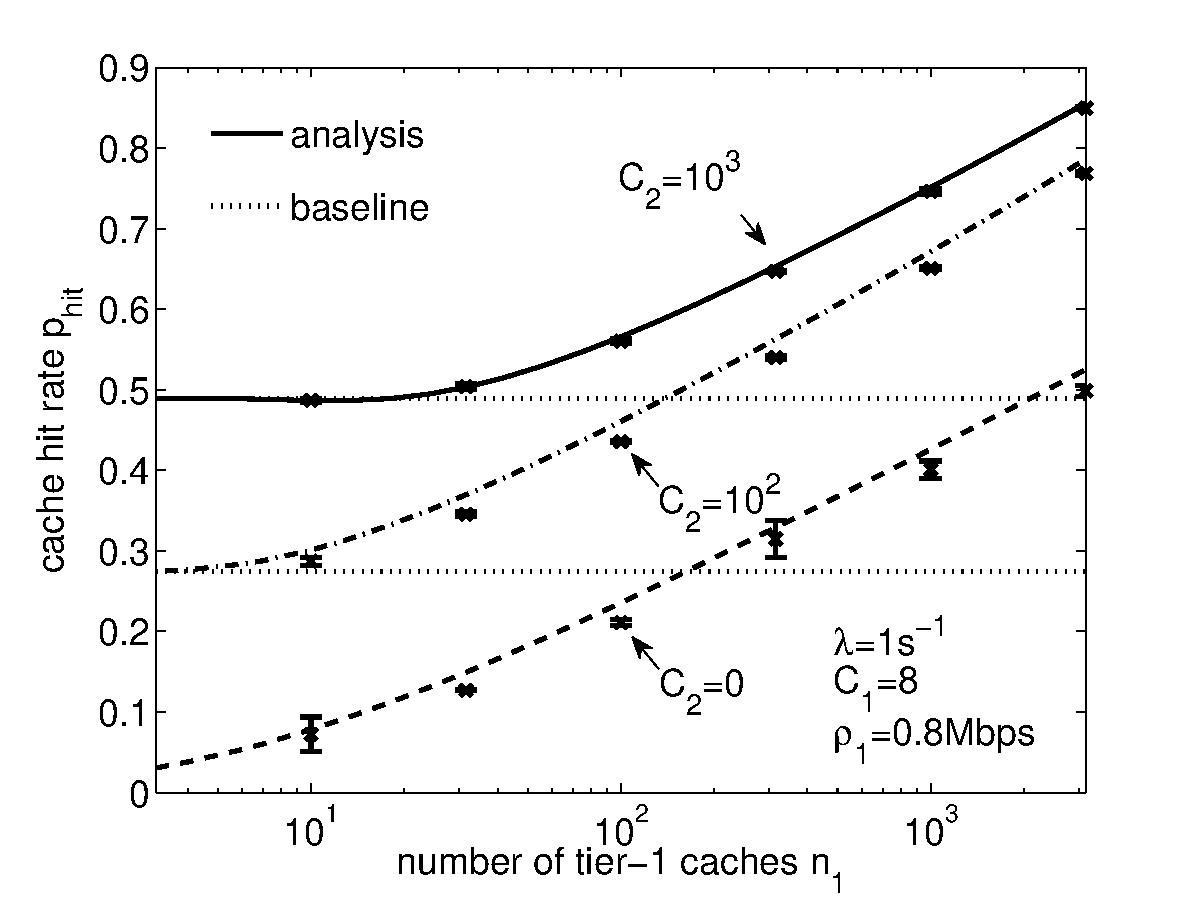
\includegraphics[width=\textwidth]{hierarchical/analyticbw/figures/hwc_l1C8_C2}
  \caption{Cache hit rate dependent on the number of tier-1 caches for different tier-2 cache capacities.}
  \label{fig:hwc_l1C8_C2}
\end{minipage}
% \hspace{0.01\textwidth}
% \begin{minipage}[b]{0.32\textwidth}
%   \centering
%   \includegraphics[width=1\textwidth]{hierarchical/analyticbw/figures/hwc_C8C1e3_l0}
%   \caption{Cache hit rate dependent on the number of tier-1 caches for varying request rates $\lambda$.}
%   \label{fig:hwc_C8C1e3_l}
% \end{minipage}
\end{figure*}

% \begin{figure}[tb]
% \centering
% 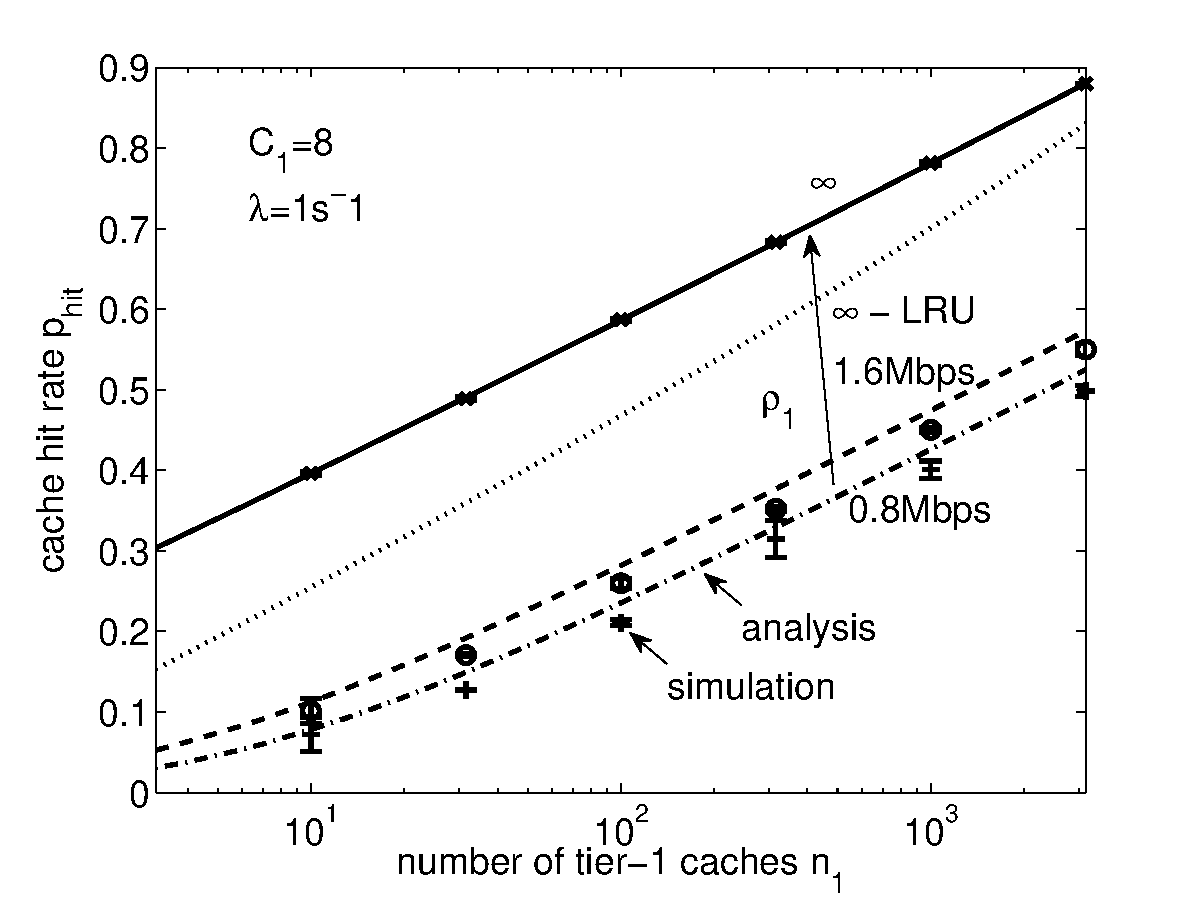
\includegraphics[width=75mm]{hierarchical/analyticbw/figures/hwc_CISP0}
% \caption{Cache hit rate dependent on number of tier-1 caches. Comparison of optimal placement with LRU policy.}
% \label{fig:hwc_CISP0}
% \end{figure}
% \begin{figure}[tb]
% \centering
% 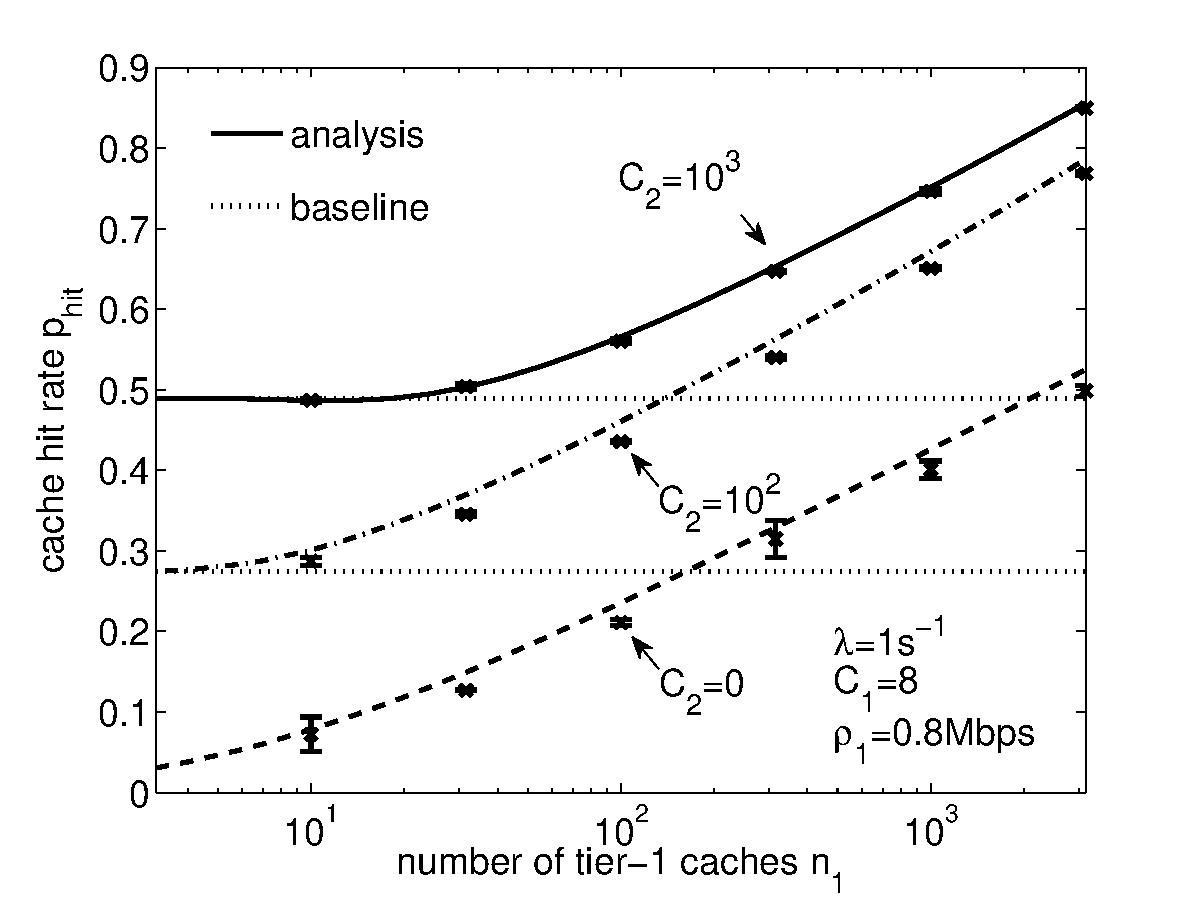
\includegraphics[width=75mm]{hierarchical/analyticbw/figures/hwc_l1C8_C2}
% \caption{Cache hit rate dependent on the number of tier-1 caches for different tier-2 cache capacities.}
% \label{fig:hwc_l1C8_C2}
% \end{figure}
% \begin{figure}[tb]
% \centering
% \includegraphics[width=75mm]{hierarchical/analyticbw/figures/hwc_C8C1e3_l0}
% \caption{Cache hit rate dependent on the number of tier-1 caches for varying request rates $\lambda$.}
% \label{fig:hwc_C8C1e3_l}
% \end{figure}

\begin{figure*}[bt]
\begin{minipage}[t]{0.49\textwidth}
  \centering
  \includegraphics[width=\textwidth]{hierarchical/analyticbw/figures/hwc_C8C1e3_l0}
  \caption{Cache hit rate dependent on the number of tier-1 caches for varying request rates $\lambda$.}
  \label{fig:hwc_C8C1e3_l}
\end{minipage}
\hspace{0.01\textwidth}
\begin{minipage}[t]{0.49\textwidth}
  \centering
  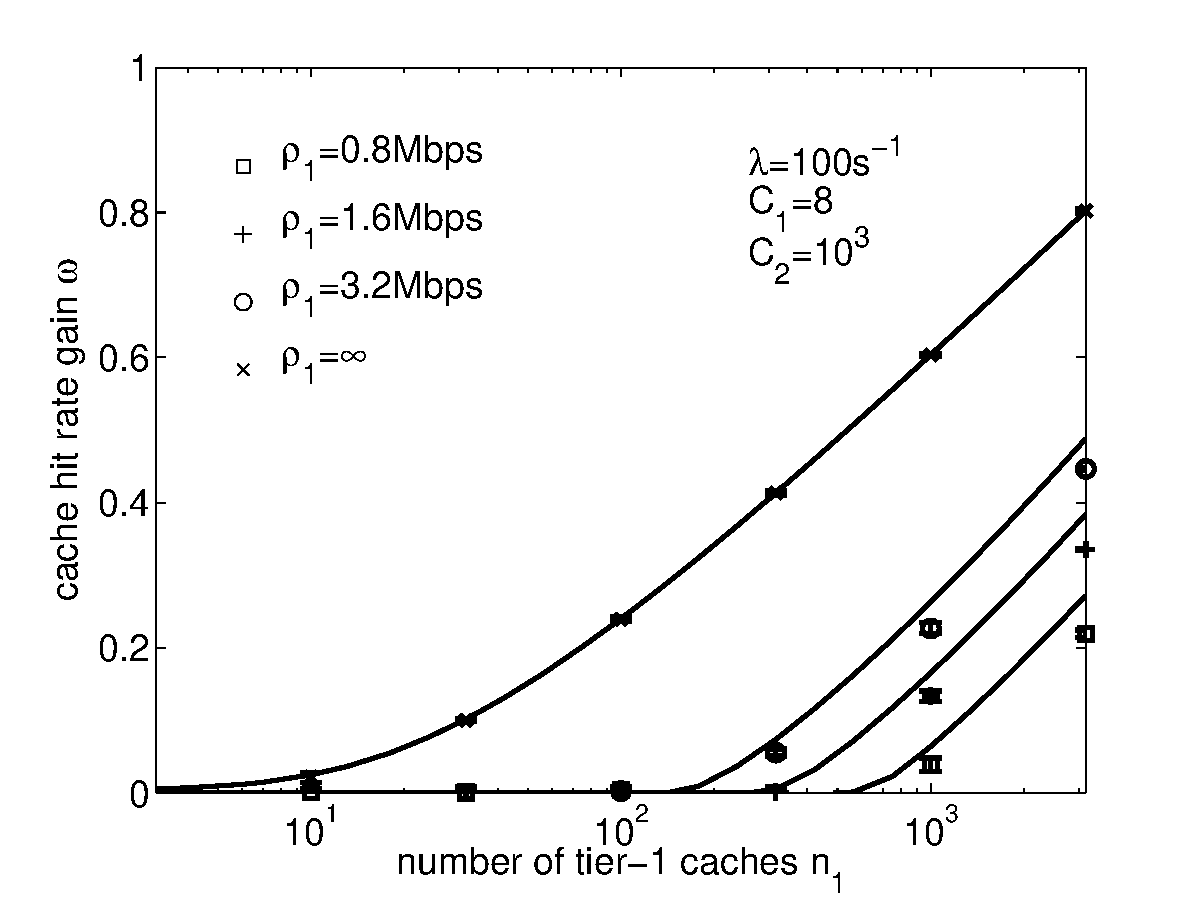
\includegraphics[width=\textwidth]{hierarchical/analyticbw/figures/hwc_C8l100_gain}
  \caption{Impact of the upload bandwidth $\rho_1$ on the cache hit rate gain $\omega$.}
  \label{fig:hwc_C8l100_gain}
  \end{minipage}
\end{figure*}

We first consider a scenario without tier-2 cache.
In this case the caching architecture only consists of tier-1 caches.
We evaluate the cache hit rate dependent on the number of tier-1 caches $n_1$.
Figure~\ref{fig:hwc_CISP0} shows the results for different upload bandwidth of tier-1 caches $\rho_1$.
The cache hit rate increases with the number of tier-1 caches and their upload bandwidth.
The analytic model slightly overestimates the cache hit rate for finite upload bandwidth of tier-1 caches.
In the case of infinite upload bandwidth, the results can be compared to an LRU cache with capacity $n_1 C_1$.
In the optimal placement, the items that are most frequently requested are placed on the caches, which explains the higher hit rate compared to LRU.

% \begin{figure}[tb]
% \centering
% \includegraphics[width=75mm]{figures/hwc_C8C1e3_l0}
% \caption{Cache hit rate dependent on the number of tier-1 caches for varying request rates $\lambda$.}
% \label{fig:hwc_C8C1e3_l}
% \end{figure}

% \begin{figure}[tb]
% \centering
% 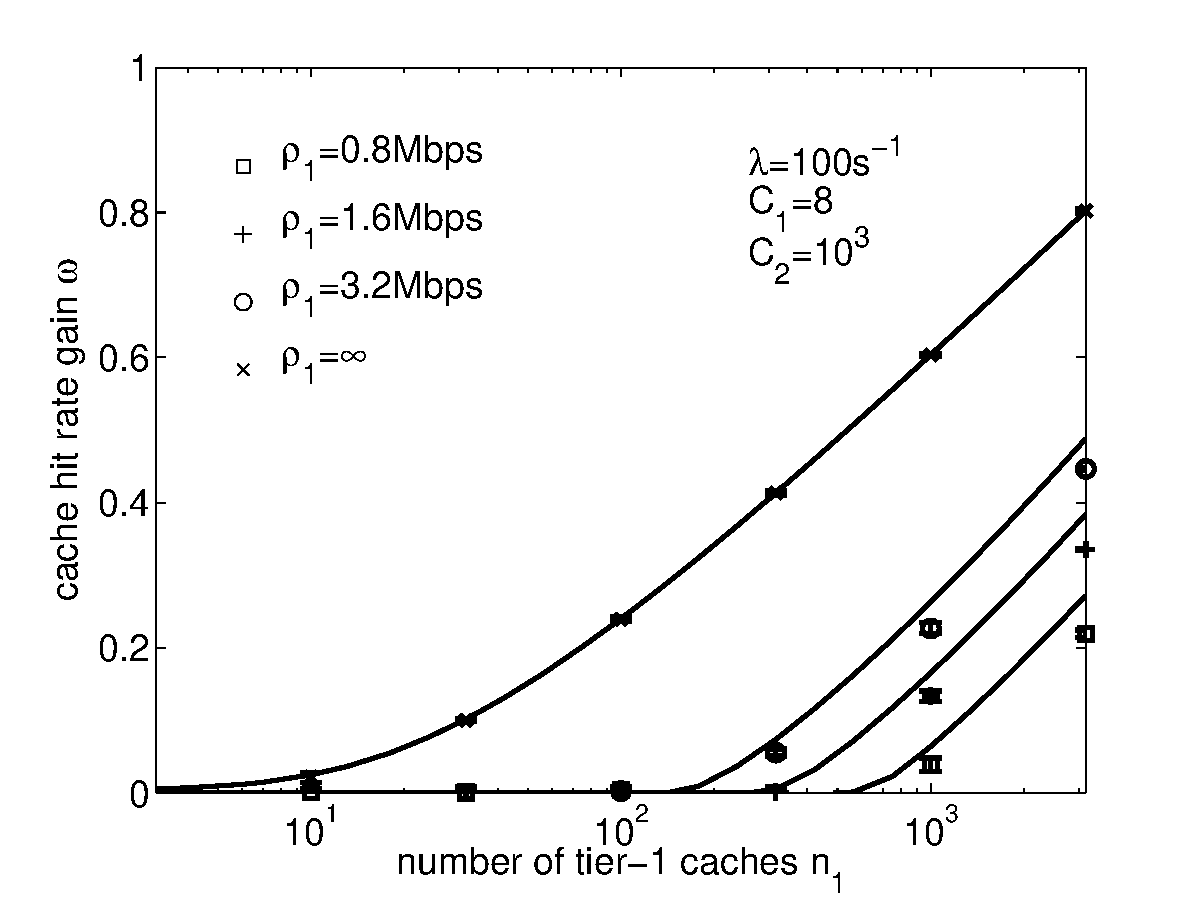
\includegraphics[width=70mm]{hierarchical/analyticbw/figures/hwc_C8l100_gain}
% \caption{Impact of the upload bandwidth $\rho_1$ on the cache hit rate gain $\omega$.}
% \label{fig:hwc_C8l100_gain}
% \end{figure}

To investigate the influence of the tier-2 cache on the cache hit rate, we vary the tier-2 cache capacity $C_2$.
Figure~\ref{fig:hwc_l1C8_C2} depicts the hit rate of the tiered caching architecture dependent on the number of tier-1 caches for different tier-2 cache capacities.
As baselines the cache hit rate $p'_\text{hit}(2)$ of a single tier-2 cache with capacity $C_2$ without tier-1 support is depicted.
The overall hit rate increases with the tier-2 cache capacity.
%If a high tier-2 cache capacity is available the number of tier-1 caches necessary to increase the performance of the tiered caching architecture is higher.

The performance of the caching architecture also highly depends on the overall request rate $\lambda$.
Figure~\ref{fig:hwc_C8C1e3_l} shows the cache hit rate dependent on the number of tier-1 caches for varying request rates $\lambda$.
Due to the limited upload bandwidth of tier-1 caches, more requests are blocked and forwarded to the tier-2 cache, which reduces the total rate of requests hit and served by tier-1 and tier-2 caches.
If the request rate increases, more tier-1 caches are necessary to increase the overall hit rate.
%For a rate of 100 requests per second, $10^3$ tier-1 caches are necessary to slightly increase the hit rate in this case.

In order to evaluate the performance of the tiered caching architecture for a medium sized ISP, we consider a high request rate $\lambda=100s^{-1}$ and a high tier-2 cache capacity $C_2=10^3$.
We study the impact of the upload bandwidth of tier-1 caches on the cache hit rate gain $\omega$.
If the upload bandwidth of the caches is low, a high number of tier-1 caches is necessary to improve the performance of the caching architecture.
The number of tier-1 caches necessary to gain hit rate decreases with their upload bandwidth.

Hence, if no tier-2 cache or only a small tier-2 cache is available, the system benefit depends on the number and bandwidth of tier-1 caches available.
In larger ISPs where a large tier-2 cache is available and where the request rate of items is high, the approach is only beneficial if the number or upload bandwidth of tier-1 caches is high enough.

%\begin{figure}[tb]
%\centering
%\includegraphics[width=75mm]{figures/ana_sim_all}
%\caption{TODO AS-Rank}
%\label{fig:ana_sim_all}
%\end{figure}
